\documentclass[fleqn]{beamer}


% \usepackage{CJKnumb}\usepackage{beamerthemesplit}

\mode<article>
{
  \usepackage{beamerbasearticle}
  \usepackage{fullpage}
  \usepackage{hyperref}
}

\usepackage{algorithm}
\usepackage{algorithmic}
\usepackage{appendixnumberbeamer}
\usepackage{color, colortbl}
\usepackage{amstext}
\usepackage{relsize}

%\usepackage{beamerthemesplit} 
%\usepackage{beamerthemeshadow}  
%\usepackage[width=2cm,dark,tab]{beamerthemesidebar}


% Setup appearance:

%\usetheme{Darmstadt}
\usefonttheme[onlylarge]{structurebold}
\setbeamerfont*{frametitle}{size=\normalsize,series=\bfseries}
\setbeamertemplate{navigation symbols}{}

\renewcommand\arraystretch{1.5}

% Standard packages

\usepackage[english]{babel}
%\usepackage[latin1]{inputenc}

\usepackage{epsf}
\usepackage{amsmath,amssymb}
\usepackage{graphicx}
\usepackage{tabularx}
\usepackage{hyperref}
\usepackage{movie15}
% \usepackage{media9}

% \usepackage[usenames,dvipsnames]{color}
\definecolor{shadow}{gray}{0.8}
\newcommand{\redc}[1]{{\color{red} #1}}
\newcommand{\bluec}[1]{{\color{blue} #1}}
\newcommand{\shadowc}[1]{{\color{shadow} #1}}
\newcommand{\blackc}[1]{{\color{black} #1}}
\newcommand{\whitec}[1]{{\color{white} #1}}
\definecolor{myyellow}{HTML}{FFB700}
\newcommand{\yellowc}[1]{{\color{myyellow} #1}}
\newcommand{\greenc}[1]{{\color{green} #1}}
\newcommand{\vect}[1]{\textbf{\textit{#1}}}
\newcommand{\dd}[0]{\textrm{d}}
\newcommand{\corr}{C^{(3)}}
\newcommand{\fe}{u}

\newcommand{\mh}{\mathcal H}
\newcommand{\eps}{\varepsilon}
\newcommand{\ml}{\mathcal L}
\newcommand{\mt}{\mathcal T}
\newcommand{\mo}{\mathcal O}
\newcommand{\mi}{\mathcal I}
\newcommand{\mc}{\mathcal C}
\newcommand{\pathmeas}{\mathcal P}
\newcommand{\proj}{\mathit\Pi}
\newcommand{\fwg}{{\mathcal A}}
\newcommand{\bwg}{{\mathcal B}}
\newcommand{\bsigma}{\boldsymbol\sigma}
\newcommand{\inv}{\textrm{inv}}

\usepackage{amsfonts}
\newcommand{\tickYes}{\checkmark}
\usepackage{pifont}
\newcommand{\tickNo}{\hspace{1pt}\ding{55}}


\definecolor{MyGray}{gray}{0.85}
\usepackage{array}
\newcolumntype{L}[1]{>{\raggedright\let\newline\\\arraybackslash\hspace{0pt}}m{#1}}
\newcolumntype{C}[1]{>{\centering\let\newline\\\arraybackslash\hspace{0pt}}m{#1}}
\newcolumntype{R}[1]{>{\raggedleft\let\newline\\\arraybackslash\hspace{0pt}}m{#1}}


\usetheme{Boadilla}
% \usetheme{Copenhagen}
% \usetheme{Madrid}
% \usetheme{Singapore}


\begin{document}
\title[Response theory for nonequilibrium system]{
  Linear response theory and optimal control for a molecular system under nonequilibrium conditions
}
%
\author{Han Wang}
\institute[FUB] {
  Institute for Mathematics, Freie Universit\"at Berlin, Germany\\
  % Institut f\"ur Mathematik, Freie Universit\"at Berlin, Germany\\
\vskip 0.4cm
Joint with: Carsten Hartmann (FUB), Christof Sch\"utte (FUB \& ZIB)}
\date[Sept. 2013]{SciCADE 2013, Valladolid}

\frame{\titlepage}

\begin{frame}{Linear response thoery for equilibrium system}{A brief review}
  \begin{itemize}
  \item <1->
    The Langevin equation under external perturbation
    \bluec{$\eps \delta\fe(t) \vect D(\vect q)$}:
    \bluec{
      \begin{align*}
        \dot{\vect q} & = \nabla_{\vect p}\mh(\vect q,\vect p), \\
        \dot{\vect p} & =- \nabla_{\vect q}\mh(\vect q,\vect p)
        + \eps \delta\fe(t) \vect D(\vect q) 
        - \gamma\vect p
        + \sigma\dot{\vect W}.
      \end{align*}
    }
  \item <2->
    The corresponding Kolmogorov forward equation:
    \bluec{
      \begin{align*}
        \frac{\partial}{\partial t} f^\eps(\vect x, t) - \fwg^\eps(t) f^\eps(\vect x, t) = 0
      \end{align*}
    }
    with forward infiniesimal generator \bluec{$\fwg^\eps (t)$}, phase space
    probability density \bluec{$f^\eps(\vect x, t)$} and phase space notation
    \bluec{$\vect x  = (\vect q, \vect p)$}.
  \end{itemize}
\end{frame}

\begin{frame}{Linear response thoery for equilibrium system}{A brief review}
  \begin{itemize}
  \item <1-> Splitting the generator:
    \bluec{
      \begin{align*}
        \fwg^\eps(t) = \fwg_0 + \eps\fwg_q(t),
      \end{align*}
    }
    where
    \bluec{
      \begin{align*}
        \fwg_0 =&
        \frac{\sigma^2}2\Delta_{\vect p}
        -
        \nabla_{\vect p}\mh\cdot\nabla_{\vect q}
        - \big(
        -\nabla_{\vect q}\mh - \gamma\vect p
        \big)\cdot\nabla_{\vect p}
        + 3N\gamma,\\
        \fwg_1(t) =&
        - \delta\fe(t) \, \vect D \cdot\nabla_{\vect p}.        
      \end{align*}
    }
  \item <2-> The asymptotic expansion of \bluec{$f^\eps$} in \bluec{$\eps$}:
    \bluec{
      \begin{align*}
        f^\eps(\vect x, t) &= f_0(\vect x, t) + \eps f_1(\vect x, t)
        +\eps^2 f_2(\vect x, t) + \mo (\eps^3),        
      \end{align*}
    }
  \end{itemize}
\end{frame}


\begin{frame}{Linear response thoery for equilibrium system}{A brief review}
  \begin{itemize}
  \item <1-> Inserting the expansion of
    \bluec{$\fwg^\eps$} and \bluec{$f^\eps(\vect x, t)$} into the
    Kolmogorov forward equation, matching different orders of \bluec{$\eps$}:
    \bluec{
      \begin{align*}
        \bigg[ \frac{\partial}{\partial t} - \fwg_0 \bigg]
        f_0(\vect x, t) = 0
      \end{align*}
    }
    Higher orders:
    \bluec{
      \begin{align*}
        \bigg[
        \frac{\partial}{\partial t}
        - \fwg_0
        \bigg]
        f_1(\vect x, t)
        =&
        \fwg_1(t) f_0(\vect x, t)\\\label{eqn:e-o2}
        \bigg[
        \frac{\partial}{\partial t}
        - \fwg_0
        \bigg]
        f_2(\vect x, t)
        =&
        \fwg_1(t) f_1(\vect x, t)        
      \end{align*}
    }
  \end{itemize}
\end{frame}

\begin{frame}{Linear response thoery for equilibrium system}{A brief review}
  \begin{itemize}
  \item <1-> Formal solution:
    \bluec{
      \begin{align*}
        f_0(\vect x, t)
        =&\,
        e^{t\fwg_0}f_0(\vect x, 0) \\
        f_1(\vect x, t)
        =&\,
        \int_0^t\dd s\,
        e^{(t-s)\fwg_0}\circ
        \fwg_1(s) f_0(\vect x,s)\\
        f_2(\vect x, t)
        =&\,
        \int_0^t\dd s\,
        e^{(t-s)\fwg_0}\circ
        \fwg_1(s) f_1(\vect x,s) 
      \end{align*}
    }
  \item <2-> Provide the initial condition being the invariant measure, i.e.
    \bluec{$f_0(\vect x, 0) = f_{\inv}(\vect x)$},
    \bluec{
      \begin{align*}
        f_0(\vect x, t) &= f_{\inv} (\vect x)\\
        f_1(\vect x, t) &=
        -\beta
        \int_0^t\dd s\,
        \delta\fe(s)\,
        e^{(t-s)\fwg_0}
        \big[
        j(\vect x)
        f_{\inv}(\vect x)
        \big]
      \end{align*}
    }
    {dissipative flux} is defined by \bluec{$j(\vect x)=-\vect D\cdot\nabla_{\vect p}\mh$}.
  \end{itemize}
\end{frame}


\begin{frame}
  \frametitle{Linear response thoery for nonequilibrium system}
  \framesubtitle{A brief review}
  \begin{itemize}
    \vfill
  \item <1-> We are interested in the observable of the system:
    \bluec{
      \begin{align*}
        \mo^\eps(t)= \int\dd \vect x \:O(\vect x)\cdot f^\eps(\vect x, t)
      \end{align*}}
    \vfill
  \item<2-> Insert
    \bluec{
      \begin{align*}
        f^\eps (\vect x, t) = f^0(\vect x, t) + \eps f^1(\vect x, t)        
      \end{align*}
    }
    \vfill
  \end{itemize}
\end{frame}


    % We denote \bluec{$\mo^0 = \int\dd \vect x O(\vect x)\cdot f_{\inv} $}
\begin{frame}{Linear response thoery for equilibrium system}{A brief review}
  \begin{itemize}
    \vfill
  \item <1-> By the previous results on the asymptotic expansion,
    we have the well-known Green-Kubo relation:
    \bluec{
      \begin{align*}
        \mo^\eps(t) = 
        \mo^0
        -
        \eps\beta
        \int_0^t\dd s\,
        \delta\fe(t-s)
        \bluec{
        \int \dd \vect x\,
        f_{\inv}(\vect x)\,
        j(\vect x)\,
        \mathbb E_{\vect x} [O(\vect x_s)]}
      \end{align*}
    }
    \bluec{$\vect x_s$}: solution to the \redc{equilibrium} Langevin eqn. with \bluec{$\vect x_0 = \vect x$}.
    \vfill
  \item[] <2-> \whitec{Last integral: {Equilibrium time correlation function} or {response function}.}
    \vfill
  \end{itemize}
\end{frame}

    % We denote \bluec{$\mo^0 = \int\dd \vect x O(\vect x)\cdot f_{\inv}$}
\begin{frame}{Linear response thoery for equilibrium system}{A brief review}
  \addtocounter{framenumber}{-1}
  \begin{itemize}
    \vfill
  \item <1-> By the previous results on the asymptotic expansion,
    we have the well-known Green-Kubo relation:
    \bluec{
      \begin{align*}
        \mo^\eps(t) = 
        \mo^0
        -
        \eps\beta
        \int_0^t\dd s\,
        \delta\fe(t-s)\redc{
        \int \dd \vect x\,
        f_{\inv}(\vect x)\,
        j(\vect x)\,
        \mathbb E_{\vect x} [O(\vect x_s)]}
      \end{align*}
    }
    \bluec{$\vect x_s$}: solution to the \redc{equilibrium} Langevin eqn. with \bluec{$\vect x_0 = \vect x$}.
    \vfill
  \item <1-> Last integral: \redc{Equilibrium time correlation function} or \redc{response function}.
    \vfill
    \end{itemize}
\end{frame}


\begin{frame}{Linear response thoery for equilibrium system}{Limitations}
  \begin{itemize}\itemsep 1cm
  \item <1-> Worse results for larger perturbation \bluec{$\eps$}.
  \item <2-> Not easy to derive higher orders of responses.
  \end{itemize}
\end{frame}



\begin{frame}{Linear response thoery for nonequilibrium system}{Driven Langevin dynamics}
  \begin{itemize}
  \item <1-> Nonequilibrium
    Langevin eqn. with external driving \bluec{$\fe(t)\,\vect D(\vect q)$}.
    \bluec{
      \begin{align*}
        \dot{\vect q} & = \nabla_{\vect p}\mh(\vect q,\vect p), \\
        \dot{\vect p} & =- \nabla_{\vect q}\mh(\vect q,\vect p)
        + \fe(t)\, \vect D(\vect q)
        - \gamma\vect p
        + \sigma\dot{\vect W},
      \end{align*}
    }
  \item <2-> 
    The perturbation to the system is \redc{$\eps\,\delta \fe(t)\,\vect D(\vect q)$}
    \bluec{
      \begin{align*}
        \dot{\vect q} & = \nabla_{\vect p}\mh(\vect q,\vect p), \\
        \dot{\vect p} & =- \nabla_{\vect q}\mh(\vect q,\vect p)
        + [\,\fe(t)\redc{ \:+\: \eps\,\delta \fe(t)}\,]\, \vect D(\vect q)
        - \gamma\vect p
        + \sigma\dot{\vect W},
      \end{align*}
    }
  \end{itemize}
\end{frame}


\begin{frame}{Linear response thoery for nonequilibrium system}{Driven Langevin dynamics}
  \begin{itemize}
  \item <1-> The nonequilibrium time dependent observable:
    \bluec{
      \begin{align*}
        \mo^\eps(t) = \langle O\,\rangle_{\pathmeas^\eps}
        = \int \dd \vect x\, f(\vect x, 0)
        \int_{\mc\{\vect x,0; t\}} O[\vect x_s]\,\dd \pathmeas^\eps[\vect x_s]
      \end{align*}
    }
    \bluec{$f(\vect x, 0)$}: The inital distribution.
    \bluec{$\mc\{\vect x,0; t\}$}: The set of all continuous trajectories starting at $\vect x$ at time 0, and stoping at time $t$.
    \bluec{$\pathmeas^\eps[\vect x_s]$}: Probability measure of trajectories.   
    \bluec{$O[\vect x_s]$}: Observable, can be functional.
  \end{itemize}
\end{frame}



\begin{frame}{Linear response thoery for nonequilibrium system}
  {The Girsanov transformation}
  \begin{itemize}
  \item <1-> The trajectory reweighting:
    \bluec{
      \begin{align*}
        \mo^\eps(t)
        &= \int \dd \vect x\, f(\vect x, 0)
        \int_{\mc\{\vect x,0; t\}} O[\vect x_s]\,\dd \pathmeas^\eps[\vect x_s]\\
        &= \int \dd \vect x\, f(\vect x, 0)
        \int_{\mc\{\vect x,0; t\}} O[\vect x_s]\,
        \frac{\dd\pathmeas^\eps[\vect x_s]}{\dd\pathmeas^0[\vect x_s]}\,
        \dd\pathmeas^0[\vect x_s]
      \end{align*}
    }
  \item<2-> The \redc{Girsanov transform}:
    \bluec{
      \begin{align*}
        \frac{\dd\pathmeas^\eps[\vect x_s]}{\dd\pathmeas^0[\vect x_s]}
        =
        \exp
        \Big[\:&
        \frac{\eps}\sigma\int_0^t
        \delta\fe(s)\,\vect D(\vect q_s)\cdot\dd\vect W_s\\
        &-
        \frac {\eps^2}{2\sigma^2}\int_0^t
        \delta\fe^2(s)\,\vect D^2(\vect q_s)\,\dd s\:
        \Big]
      \end{align*}
    }
  \end{itemize}
\end{frame}


        % + \eps\:
        % \Big\langle
        % O[\vect x_s]\cdot \frac{1}\sigma\int_0^t
        % \delta\fe(s)\,\vect D(\vect q_s)\cdot\dd\vect W_s
        % \Big\rangle_{\pathmeas^0}

\begin{frame}{Linear response thoery for nonequilibrium system}
  {The linear and quadratic approximation}
  \begin{itemize}
  \item<1-> Linear approximation of exponent:
    \bluec{
      \begin{align*}
        \mo^\eps(t) \approx\: & \mo^0(t)\\
        &+
        \redc{\eps\:
          \Big\langle
          O[\vect x_s]\cdot G[\vect x_s]
          \Big\rangle_{\pathmeas^0}}
        \\
        &+
        \redc{
        \frac{\eps^2}2\:
        \Big\langle
        O[\vect x_s]\cdot \big\{\, G[\vect x_s]^2 - H[\vect x_s]\,\big\}
        \Big\rangle_{\pathmeas^0}}
      \end{align*}
    }
  \item<2-> where
    \bluec{
      \begin{align*}
        G[\vect x_s] & = \int_0^t\frac 1\sigma\,\delta\fe(s)\,\vect D(\vect q_s)\cdot \dd\vect W_s\\
        H[\vect x_s] & = \int_0^t\frac 1{\sigma^2}\,\delta\fe^2(s)\,\vect D^2(\vect q_s)\cdot \dd s
    \end{align*}
    }
  \end{itemize}
\end{frame}


\begin{frame}{Numerical example: splitting single well potentialu}
  \begin{itemize}
  \item<1-> Single well Hamiltonian:
    \bluec{
      \begin{align*}
        H(\vect q, \vect p) = \frac12\vert \vect p\vert^2 + \frac12 k\vert \vect q\vert^2
      \end{align*}
    }
  \item<2-> External drive:
    \bluec{
      \begin{align*}
        u(t)\vect D(\vect q) = - k_e \frac{t}{T}\cdot
        \nabla_{\vect q}
        \Big[
        \frac{1}{\sqrt{2\pi \Sigma^2}} \exp\Big\{-\frac{ q^2}{2\Sigma^2}\Big\}
        \Big]
      \end{align*}
    }
  \item<3-> Perturbation:
    \bluec{
      \begin{align*}
        \eps\delta u(t)\vect D(\vect q) = - \eps\cdot k_e \frac{t}{T}\cdot
        \nabla_{\vect q}
        \Big[
        \frac{1}{\sqrt{2\pi \Sigma^2}} \exp\Big\{-\frac{ q^2}{2\Sigma^2}\Big\}
        \Big]        
      \end{align*}
    }
  \end{itemize}
\end{frame}


\begin{frame}{Numerical example: splitting single well potential}
  \begin{figure}
    \includegraphics[width=0.8\textwidth]{figs/drive/frame-10.eps}
  \end{figure}  
\end{frame}

\begin{frame}{Numerical example: splitting single well potential}
  \addtocounter{framenumber}{-1}
  \begin{figure}
    \includegraphics[width=0.8\textwidth]{figs/drive/frame-01.eps}
  \end{figure}  
\end{frame}

\begin{frame}{Numerical example: splitting single well potential}
  \addtocounter{framenumber}{-1}
  \begin{figure}
    \includegraphics[width=0.8\textwidth]{figs/drive/frame-02.eps}
  \end{figure}  
\end{frame}

\begin{frame}{Numerical example: splitting single well potential}
  \addtocounter{framenumber}{-1}
  \begin{figure}
    \includegraphics[width=0.8\textwidth]{figs/drive/frame-10.eps}
  \end{figure}  
\end{frame}

\begin{frame}{Numerical example: splitting single well potential}
  \addtocounter{framenumber}{-1}
  \begin{figure}
    \includegraphics[width=0.8\textwidth]{figs/drive/frame-11.eps}
  \end{figure}  
\end{frame}

\begin{frame}{Numerical example: splitting single well potential}
  \addtocounter{framenumber}{-1}
  \begin{figure}
    \includegraphics[width=0.8\textwidth]{figs/drive/frame-12.eps}
  \end{figure}  
\end{frame}




\begin{frame}{Numerical example: splitting single well potential}
  The probability density on the phase space: Exnternal vedio
  \begin{figure}[ht]
    \includemovie[poster,autoplay,externalviewer]{}{}{figs/movie/fig-2d-tog.mp4}
  \end{figure}
 % \flashmovie[engine=flv-player,auto=1,controlbar=0]{/home/wanghan/study/noneq.msm/writedown/linear.response/figs/tilt.warm020.str6.0.nst1e09.smallgrid/fig-2d-tog.flv}
  % /home/wanghan/study/noneq.msm/writedown/linear.response/figs/tilt.warm020.str6.0.nst1e09.smallgrid/fig-2d-tog.mp4
\end{frame}

\begin{frame}{Numerical example: splitting single well potential}
  \begin{figure}
    \includegraphics[width=0.7\textwidth]{figs/movie/fig-2d-tog-00020.pdf}
  \end{figure}  
\end{frame}


\begin{frame}
  \frametitle{{Optimal control of a nonequilibrium system}}
  The optimal control problem
  \bluec{
    \begin{align*}
      \max_{u\in\mathcal U} \ I&(u) = \langle\, \psi (u) \,\rangle_{\pathmeas^0}\\
      \textbf{s.t.} \quad&
        \dot{\vect q}  = \nabla_{\vect p}\mh(\vect q,\vect p), \\
        &\dot{\vect p}  =- \nabla_{\vect q}\mh(\vect q,\vect p)
        + \fe(t)\, \vect D(\vect q)
        - \gamma\vect p
        + \sigma\dot{\vect W},      
    \end{align*}
  }
  where:
  \bluec{
    \begin{align*}
      \psi(u) =
      \int_0^T
      \Big\{ f(q_s) - \frac12\vert u(s)\vert^2\Big\}\, \dd t + g(q_T)\,
    \end{align*}
  }
  \bluec{$f$} and \bluec{$g$} are the running cost and the terminal cost.
\end{frame}


\begin{frame}
  \frametitle{Optimal control of a nonequilibrium system}
  \begin{itemize}
  \item<1-> 
    Assuming the forcing is presented by:
    \bluec{
      \begin{align*}
        u(t) = \sum_{k = 1}^K a_k\Phi_k(t), \quad a_k\in \mathbb R
      \end{align*}
    }
  \item<2-> The gradient descent searching:
    \bluec{
      \begin{align*}
        u^{(n+1)} = u^{(n)} + \tau_n \,\nabla I\,(u^{(n)})
      \end{align*}
    }
  \item<3-> In the space spanned the ansatz functions:
    \bluec{
      \begin{align*}
        a_k^{(n+1)}   = a_k^{(n)} +
        \tau_n \,\frac{\partial I}{\partial a_k} \bigg\vert_{a_k = a_k^{(n)}}
      \end{align*}
    }
  \end{itemize}
\end{frame}


\begin{frame}
  \frametitle{Optimal control of a nonequilibrium system}
  \begin{itemize}
  \item<1-> With the response theory we have
    \bluec{
      \begin{align*}
        \frac{\partial I}{\partial a_k} =
        \bigg\langle
        \psi \int_0^T\frac1\sigma\,\Phi_k(s)\,\vect D(q_s)\cdot \dd W_s
        +
        \int_0^T u(s)\,\Phi_k(s)\,\dd s
        \bigg\rangle_{\pathmeas^0}
      \end{align*}
    }
  \end{itemize}
\end{frame}

\begin{frame}
  \frametitle{Optimal tilting of a double-well potential}
  \begin{itemize}
  \item<1-> 
    \begin{minipage}[t]{0.6\linewidth}
      The 1-D double-well potential:
      \bluec{
        \begin{equation*}
          U(q) = \frac k2\, (q^2 - a^2)^2
        \end{equation*}
      }
      with tilting:
      \bluec{
        \begin{align*}
          D(q) = -\nabla_q V(q) = 1
        \end{align*}
      }
    \end{minipage}
    \hfill
    \begin{minipage}[t]{0.350\linewidth}
      \begin{figure}
        \centering
        \includegraphics[width=1.0\textwidth]{figs/double.well/potential.eps}
      \end{figure}
    \end{minipage}
    \hfill
  \item<2-> The optimal forcing problem:
    \bluec{
      \begin{align*}
        I = \max_{u\in\mathcal U} I(u), \quad
        I(u) =
        \bigg\langle
        \chi(q_T\in [0,+\infty)) - \frac\eta 2\int_0^T\vert u(s)\vert^2\,\dd s
        \bigg\rangle_{\pathmeas^0}
      \end{align*}
    }
  \item<3-> \bluec{$\Phi_k(t)$}: piecewise linear function.
  \end{itemize}
\end{frame}


\begin{frame}
  \frametitle{Optimal tilting of a double-well potential}
  \begin{figure}
    \centering
    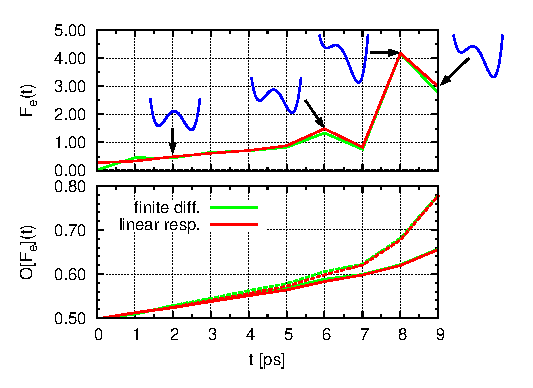
\includegraphics[width=0.8\textwidth]{figs/fig-ctr-stat-2.eps}
  \end{figure}
\end{frame}








\begin{frame}
  Thank you...
\end{frame}

\end{document}


